\documentclass[a4paper,UTF8]{article}
\usepackage{ctex}
\usepackage[margin=1.25in]{geometry}
\usepackage{color}
\usepackage{graphicx}
\usepackage{amssymb}
\usepackage{amsmath}
\usepackage{amsthm}
\usepackage{enumerate}
\usepackage{bm}
\usepackage{hyperref}
\usepackage{epsfig}
\usepackage{color}
\usepackage{mdframed}
\usepackage{lipsum}
\usepackage{mathtools}
\usepackage{hyperref}
\usepackage{diagbox}
\usepackage{float}
\usepackage{caption}
\usepackage{algorithm}
\usepackage{algorithmicx}  
\usepackage{algpseudocode}
\usepackage{amsmath} 
\usepackage{graphicx}
\usepackage{subfigure}
\newmdtheoremenv{thm-box}{myThm}
\newmdtheoremenv{prop-box}{Proposition}
\newmdtheoremenv{def-box}{定义}
\usepackage{listings}
\usepackage{xcolor}
\lstset{
	numbers=left, 
	numberstyle= \tiny, 
	keywordstyle= \color{ blue!70},
	commentstyle= \color{red!50!green!50!blue!50}, 
	frame=shadowbox, % 阴影效果
	rulesepcolor= \color{ red!20!green!20!blue!20} ,
	escapeinside=``, % 英文分号中可写入中文
	xleftmargin=2em,xrightmargin=2em, aboveskip=1em,
	framexleftmargin=2em
} 

\usepackage{booktabs}

\setlength{\evensidemargin}{.25in}
\setlength{\textwidth}{6in}
\setlength{\topmargin}{-0.5in}
\setlength{\topmargin}{-0.5in}

% \setlength{\textheight}{9.5in}
%%%%%%%%%%%%%%%%%%此处用于设置页眉页脚%%%%%%%%%%%%%%%%%%
\usepackage{fancyhdr}                                
\usepackage{lastpage}                                           
\usepackage{layout}                                             
\footskip = 10pt 
\pagestyle{fancy}                    % 设置页眉                 
\lhead{研一下学期}                    
\chead{论文阅读笔记}                                                
% \rhead{第\thepage/\pageref{LastPage}页} 
\rhead{Step6}                                                                                               
\cfoot{\thepage}                                                
\renewcommand{\headrulewidth}{1pt}  			%页眉线宽,设为0可以去页眉线
\setlength{\skip\footins}{0.5cm}    			%脚注与正文的距离           
\renewcommand{\footrulewidth}{0pt}  			%页脚线宽,设为0可以去页脚线

\makeatletter 									%设置双线页眉                                        
\def\headrule{{\if@fancyplain\let\headrulewidth\plainheadrulewidth\fi%
\hrule\@height 1.0pt \@width\headwidth\vskip1pt	%上面线为1pt粗  
\hrule\@height 0.5pt\@width\headwidth  			%下面0.5pt粗            
\vskip-2\headrulewidth\vskip-1pt}      			%两条线的距离1pt        
 \vspace{6mm}}     								%双线与下面正文之间的垂直间距              
\makeatother  

%%%%%%%%%%%%%%%%%%%%%%%%%%%%%%%%%%%%%%%%%%%%%%
\numberwithin{equation}{section}
%\usepackage[thmmarks, amsmath, thref]{ntheorem}
\newtheorem{theorem}{Theorem}
\newtheorem*{definition}{Definition}
\newtheorem*{solution}{Solution}
\newtheorem*{prove}{Proof}
\newcommand{\indep}{\rotatebox[origin=c]{90}{$\models$}}

\usepackage{multirow}

%--

%--
\begin{document}
\title{论文阅读笔记\\
Step6}
\author{MF1833063, 史鹏, spwannasing@gmail.com}
\maketitle


\newpage
\section{Cognitive Graph for Multi-Hop Reading Comprehension at Scale}
这篇文章基于Bert和GNN,在迭代中逐步构建出cognitive graph:$\mathcal{G}$,图中的每一个节点都和一个实体或者一个可能的答案有关。
由两部分组成:implicit extraction(System 1)和explicit reasoning(System 2)。

\begin{figure}[H]
	\centering
	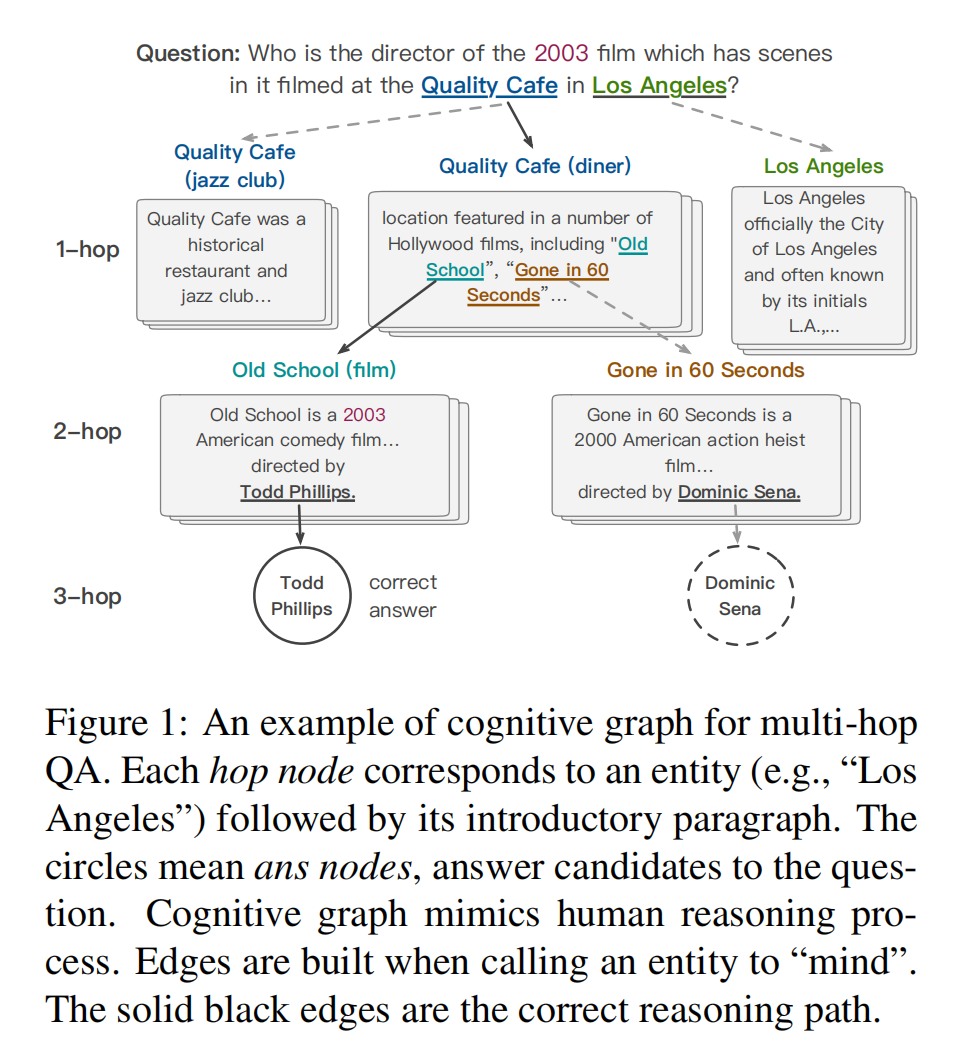
\includegraphics[width=0.5\textwidth]{1-1.png}
\end{figure}
\begin{figure}[H]
	\centering
	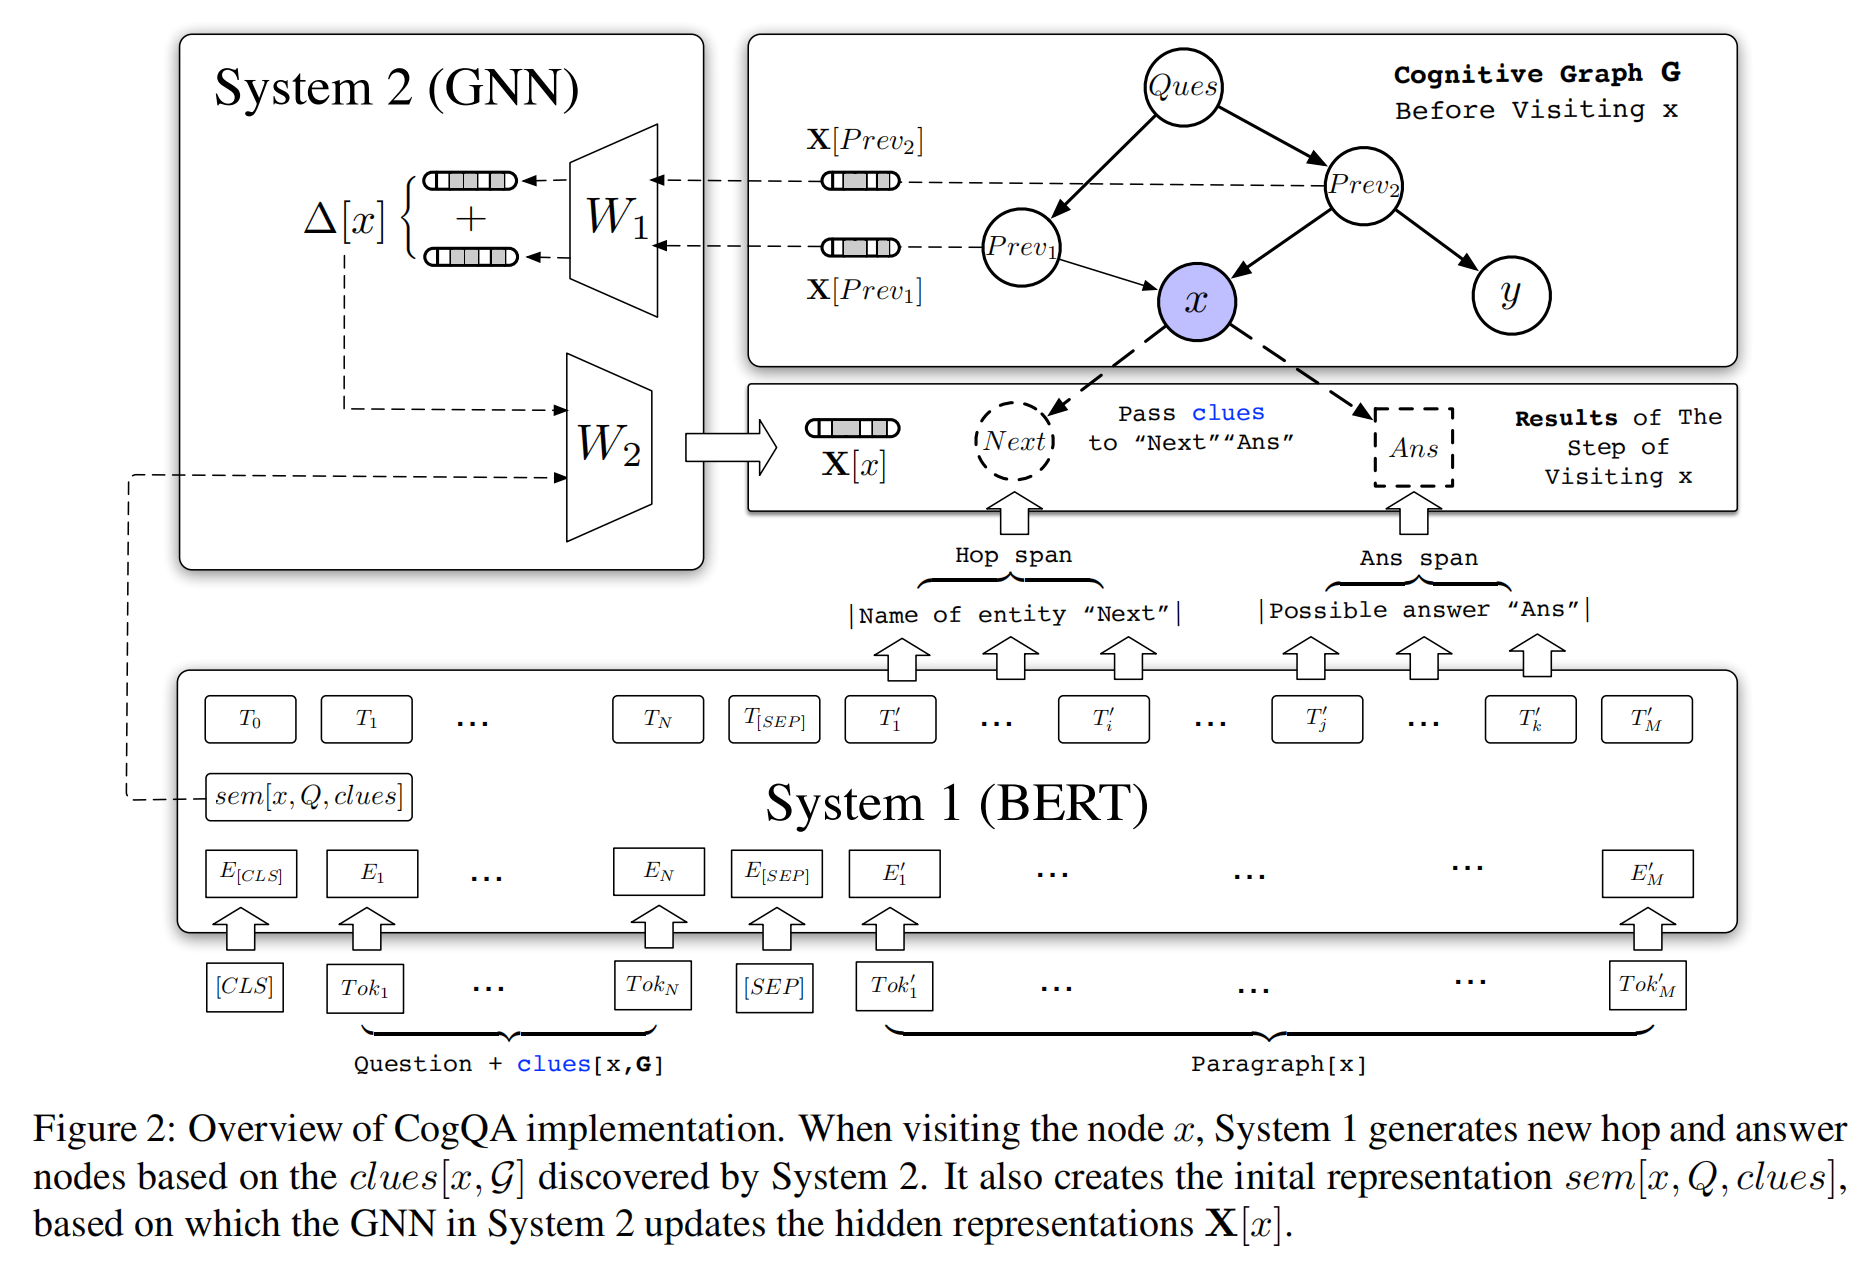
\includegraphics[width=\textwidth]{1-3.png}
\end{figure}
\begin{figure}[H]
	\centering
	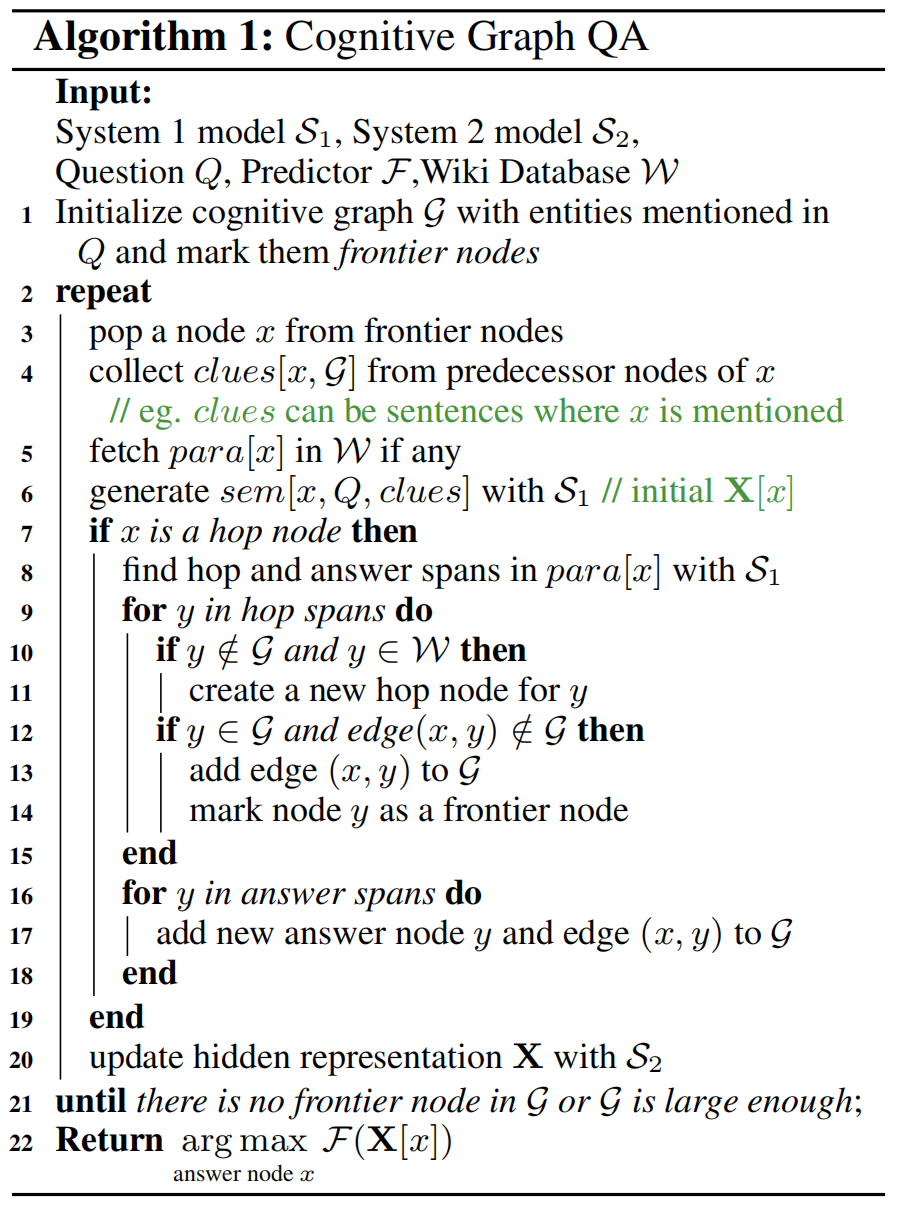
\includegraphics[width=0.5\textwidth]{1-2.png}
\end{figure}
[注] 本文选取的数据集是HotpotQA,HotpotQA 是一个大型问答数据集,它包含约 11.3 万个具备上述特征的问答对。也就是说,这些问题要求问答系统能够筛选大量的文本文档,以找到与生成答案相关的信息,并对找到的多个支撑性事实进行多步推理,从而得出最终答案。

System 1从段落中提取与问题相关的实体和answer candidate,并对其语义信息进行编码。提取的实体被组织成一个Cognitive Graph。
然后,系统2对图进行推理,并收集线索指导系统1更好地提取下一跳实体。

System 1(Bert):\\
\begin{equation}
	\underbrace{[C L S] Q u e s t i o n[S E P] \operatorname{clues}[x, \mathcal{G}][S E P]}_{\text { Sentence } A} \underbrace{\operatorname{Para}[x]}_{\text { Sentence } B}
	\end{equation}

System 2(GNN): \\
\begin{equation}
\begin{array}{l}{\Delta=\sigma\left(\left(A D^{-1}\right)^{T} \sigma\left(\mathbf{X} W_{1}\right)\right)} \\ {\mathbf{X}^{\prime}=\sigma\left(\mathbf{X} W_{2}+\Delta\right)}\end{array}
\end{equation}
\newpage
\section{Exploiting Explicit Paths for Multi-hop Reading Comprehension}
本文基于WikiHop数据集,在该数据集中问题以三元组的形式出现$\left(h_{e}, r, ?\right)$,$h_e$代表head entity,r代表head entity和未知的tail entity之间的关系。
任务是从给定的candidates集合中选出一个答案:$\left(c_{1}, c_{2}, \dots, c_{N}\right)$。

所做的工作是在预测答案的同时,将推理的path展示出来。方法很intuitive,但难的是想到并去做这个工作。
\begin{figure}[H]
	\centering
	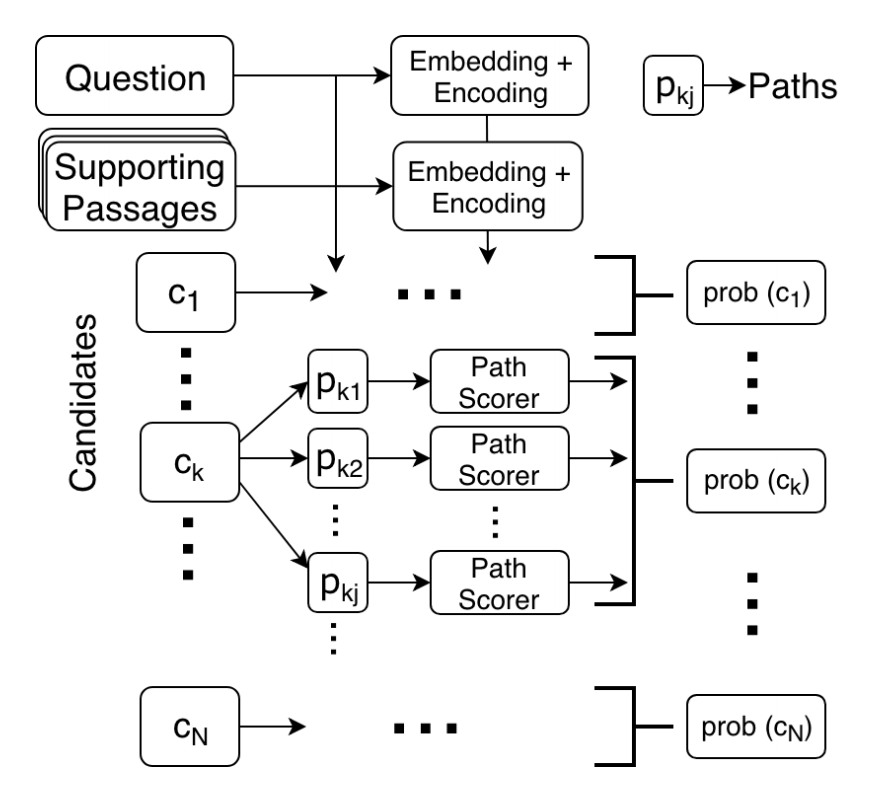
\includegraphics[width=0.6\textwidth]{2-1.png}
	\caption{Architecture of the proposed model}
\end{figure}
\begin{figure}[H]
	\centering
	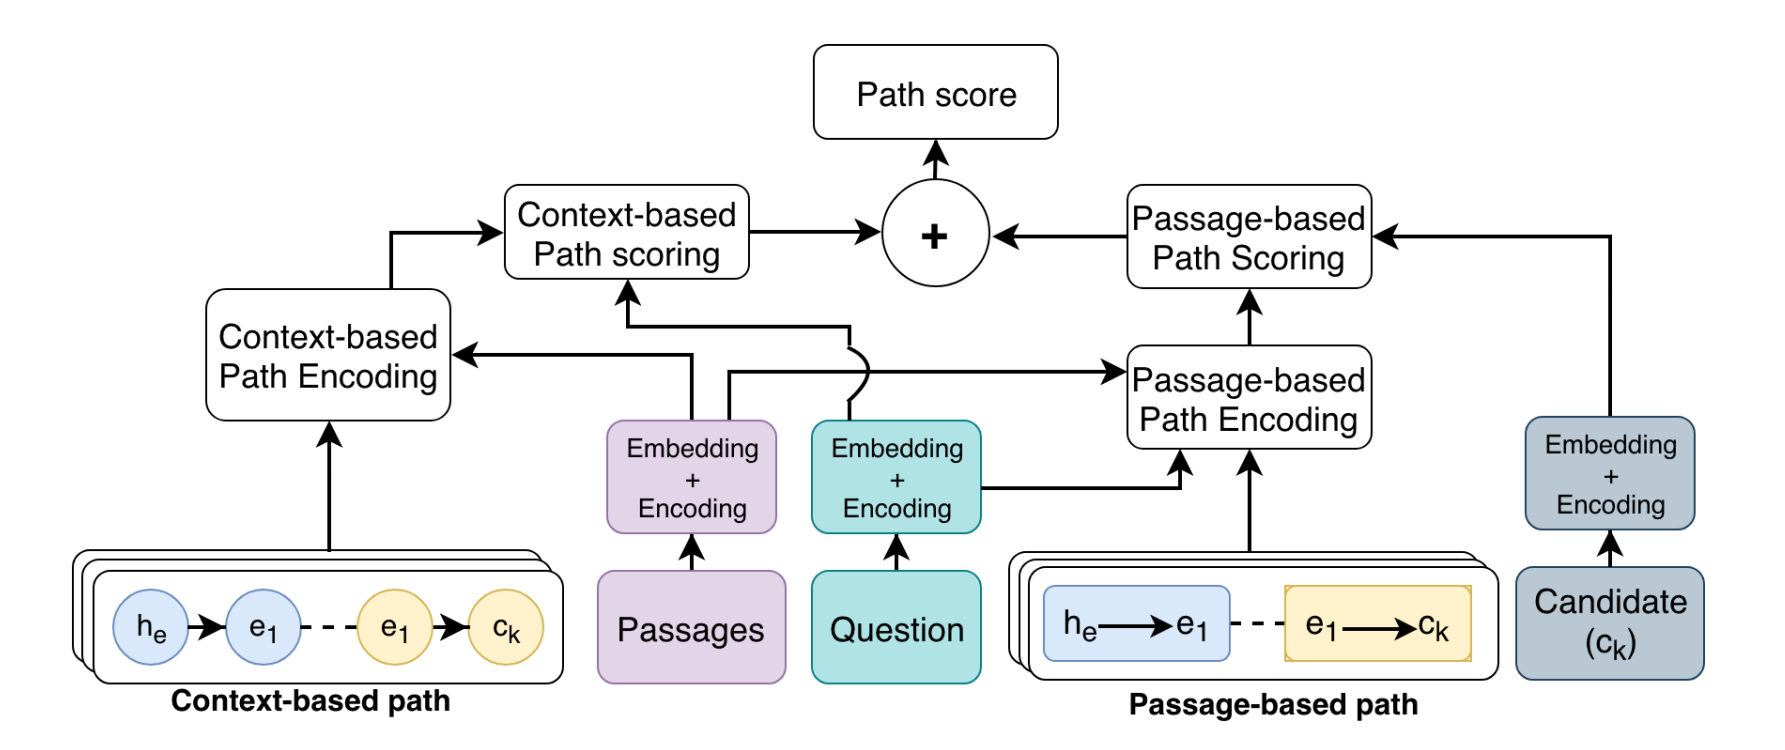
\includegraphics[width=\textwidth]{2-2.png}
	\caption{Architecture of the proposed path scoring module}
\end{figure}
\newpage
模型的流程是:
\begin{enumerate}
	\item 提取Path
	在含有$h_e$的第一篇文章中,找出在那句话或者下一句话中出现的所有实体,然后在其它的passage中寻找这些实体,如果该passge也包含candidate中的单词那么则构建出了一个path。
	为每一个candidate构建一个从$h_e$的路径。
	\item 对所有的path进行encoding以及score,选出answer以及输出path。
	\subitem[1] Context-based Path Encoding:

	对于2-hop的path:$(h_e,e_1),(e_1,c_k)$:
	\begin{equation}
		\mathbf{g}_{h_{e}}=\mathbf{s}_{p_{1}, i_{1}} \| \mathbf{s}_{p_{1}, i_{2}}
		\end{equation}
		\begin{equation}
			\mathrm{FFL}(\mathbf{a}, \mathbf{b})=\tanh \left(\mathbf{a} \mathbf{W}_{a}+\mathbf{b} \mathbf{W}_{b}\right)
			\end{equation}
		\begin{equation}
			\mathbf{r}_{h_{e}, e_{1}}=\operatorname{FFL}\left(\mathbf{g}_{h_{e}}, \mathbf{g}_{e_{1}}\right)
			\end{equation}
			\begin{equation}
				\mathbf{x}_{c t x}=\operatorname{FFL}\left(\mathbf{r}_{h_{e}, e_{1}}, \mathbf{r}_{e_{1}, c_{k}}\right)
				\end{equation}
	\subitem[2] Passage-based Path Encoding:\\
	首先计算相似矩阵:$\mathbf{A}_{p} \in \mathbb{R}^{T \times U}$,然后分别计算question-aware passage和passage-aware question:
	$\mathbf{S}_{p}^{q_{1}}=\mathbf{A Q}$和$\mathbf{Q}_{p}=\mathbf{A}^{\top} \mathbf{S}_{p}$,根据更新的question表示再计算$\mathbf{S}_{p}^{q_{2}} \in \mathbb{R}^{T \times H}$,其中$\mathbf{S}_{p}^{q_{2}}=\mathbf{A} \mathbf{Q}_{p}$

	然后将两次计算的结果拼接:$S_p^q\in \mathbb{R}^{T \times 2 H}=\mathbf{S}_{p}^{q_{1}} \| \mathbf{S}_{p}^{q_{2}}$。
	\begin{equation}
	\begin{array}{l}{a_{t}^{p} \propto \exp \left(\mathbf{s}_{p, t}^{q} \mathbf{w}^{\top}\right)} \\ {\tilde{\mathbf{s}}_{p}=\mathbf{a}^{p} \mathbf{S}_{p}^{q}}\end{array}
	\end{equation}
	\begin{equation}
		\mathbf{x}_{p s g}=\operatorname{FFL}\left(\tilde{\mathbf{s}}_{p 1}, \tilde{\mathbf{s}}_{p_{2}}\right)
		\end{equation}
	\subitem[3] Path Scoring:
	\begin{equation}
		\tilde{\mathbf{q}}=\left(\mathbf{q}_{0} \| \mathbf{q}_{U}\right) \mathbf{W}_{q}
		\end{equation}
		\begin{equation}
			\mathbf{y}_{x_{c t x}, q}=\mathrm{FFL}\left(\mathbf{x}_{c t x}, \tilde{\mathbf{q}}\right)
			\end{equation}
			\begin{equation}
				z_{c t x}=\mathbf{y}_{x_{c t x}, q} \mathbf{w}_{c t x}^{\top}
				\end{equation}
				\begin{equation}
					z_{p s g}=\tilde{\mathbf{c}}_{k} \mathbf{x}_{p s g}^{\top}
					\end{equation}
					\begin{equation}
						z=z_{c t x}+z_{p s g}
						\end{equation}
\end{enumerate}
\end{document}